\documentclass{article}
\usepackage{amsmath, indentfirst, epsfig, ifthen, booktabs, multirow}
\usepackage{nomencl}
\makenomenclature

\renewcommand{\nomgroup}[1]{%
%\ifthenelse{\equal{#1}{A}}{\item[\textbf{Roman Symbols}]}{%
\ifthenelse{\equal{#1}{G}}{\item[\textbf{Greek Symbols}]}{%
\ifthenelse{\equal{#1}{C}}{\item[\textbf{Abbreviations}]}{%
\ifthenelse{\equal{#1}{S}}{\item[\textbf{Subscripts}]}% matches mathematical symbols
}% matches Subscripts
}% matches Abbreviations
}% matches Greek Symbols
}% matches Roman Symbols

\makeindex
\begin{document}

\title{Cascade system using both trough system and dish system for power generation}
\date{}
%\author{Cheng Zhang}
\maketitle
\printnomenclature[2.5cm]{}

\newpage{}

\section{Introduction}
\begin{itemize}
    \item Background Information
    \begin{enumerate}
        \item Why do we need cascade system
        \item What is the advantage of cascade system
        \item What are others' works
        \item What have been done
        \item What to be done
        \item What can we improve
        \item What have we done
    \end{enumerate}
    \item System specification
    \begin{enumerate}
    	\item Environment
	\item Trough collector
	\item Dish collector
	\item Steam turbine
	\item Stirling engine
    \end{enumerate}
    \begin{enumerate}
    	\item Air circuit
	\item Water circuit
	\item Oil circuit
	\item System efficiency
    \end{enumerate}    
    \item Separate system
    \item Results
\end{itemize}

Different types of collectors and different technologies for electricity generation are suitable for different working temperature zones with different costs. An idea of cascade collection and cascade utilisation of solar energy with higher efficiency is presented. Parabolic trough collectors are used to collect lower temperature energy with lower cost and dish collectors are used to collect higher temperature energy with higher efficiency. Rankine cycle is used to work in lower temperature zone and Stirling cycle is used to work in higher temperature zone. Furthermore, effective topological structures are considered to take full advantages of thermodynamic characters of different components of the system. The cold chamber of Stirling engine is cooled by condensed fluid of Rankine cycle to use the heat released by Stirling engine. 

\section{System description}
An EES\nomenclature[C]{EES}{Engineering Equation Solver} model was used to study the characteristics of the cascade system. Figure~\ref{fig:System-1} shows the sketch of the cascade system. Dish collectors are used to provide heat for Stirling engines and air-to-water heat exchanger. Trough collectors are used to provide heat for preheating, evaporating and superheating in the Rankine cycle. Water is used as the working fluid of Rankine cycle, which is heated in the cold chamber of Stirling engines, preheater, evaporator, superheater, and air-to-water heat exchanger successively, and then expand in turbine, condense in condenser. Pumps are used to change the pressure of fluids. Stirling engines are used for power generation and cooled by feed water of the Rankine cycle. State number pairs of different fluids are marked on the sketch. The first number of a number pair indicates the fluid type, the second number of a number pair indicates the state point of the fluid. Number pairs with solid circle indicate saturated liquid states ($x$\nomenclature{$x$}{Dryness fraction} = 0), and with dotted circle indicates saturated gas states ($x$ = 1).

\noindent \begin{figure}[htbp]
\begin{center}
	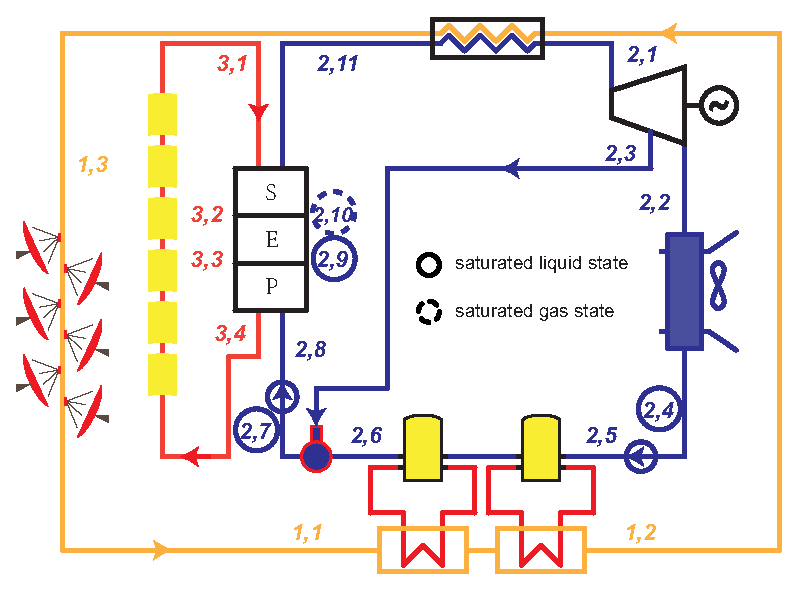
\includegraphics[width = 0.8\textwidth]{./graphics/cascadeSystem}
	\caption{Sketch of the cascade system}
	\label{fig:System-1}
\end{center}
\end{figure}

To build the cascade system model, several simplifying assumptions are made:

\begin{itemize}
	\item Steady state at nominal load of the system is analyzed
	\item Pressure drop due to flow is negligible everywhere
	\item Same isentropic efficiency of steam turbine with different loads and in different stages
	\item There is no heat loss to the environment for Stirling engines
	\item Simple models are used of some processes and equipments
	\item A symmetrical regenerator behaviour is assumed so that a single effectiveness can be defined as $e=\dfrac{T_R - T_L}{T_H - T_L}$\cite{Formosa2010, Albert2010}
	\item There is no heat loss to the environment for Stirling engines
\end{itemize}

\section{System specification}
Table~\ref{tab:system-data} shows the basic design parameters of the cascade system.

\begin{table}[htbp]
	\caption{Parameters of the cascade system}
	\begin{center}
	\begin{tabular}{cccc}
		\toprule
		\multicolumn{4}{c}{Nominal electric power}\\
		\midrule
		$P_{generator}$\nomenclature{$P_{generator}$}{Power of generator, W} & 6$\times10^6$ W\\
		\midrule
		\multicolumn{4}{c}{Environment}\\
		\midrule
		$I_{DNI}$\nomenclature{$I_{DNI}$}{Direct Normal Irradiance, W/m$^2$} & 700 W/m$^2$ & $T_{amb}\nomenclature{$T_{amb}$}{Ambient temperature, K}$ & 293 K\\
		$p_{amb}$\nomenclature{$p_{amb}$}{Ambient pressure, Pa} & 1$\times10^5$ Pa & $v_{wind}$\nomenclature{$v_{wind}$}{Ambient wind speed, m/s} & 4 m/s\\
		\midrule
		\multicolumn{4}{c}{Dish collector}\\
		\midrule
		$T_{dish,inlet}\nomenclature{$T_{dish,inlet}$}{Dish inlet temperature, K}$ & 623K & $T_{dish,outlet}$\nomenclature{$T_{dish,outlet}$}{Dish outlet temperature} & 1073 K\\
		$p_{dish}$\nomenclature{$p_{dish}$}{Air pressure in dish, Pa} & 5$\times10^5$ Pa & 	$A_{dishCollector}$\nomenclature{$A_{dishCollector}$}{Aperture area of each dish collector, m$^2$} & 87.7 m$^2$\\
		\midrule
		\multicolumn{4}{c}{Trough collector}\\
		\midrule
		$\Delta{}T_{oil,water,min}$\nomenclature[G]{$\Delta{}T_{oil,water,min}$}{Minimum temperature difference between oil and water in the oil-to-water heat exchanger, K} & 15 K &	$T_{trough,outlet}$\nomenclature{$T_{trough,outlet}$}{Trough outlet temperature} & 623 K\\
		$p_{trough}$\nomenclature{$p_{trough}$}{Air pressure in trough, Pa} & 2$\times10^6$ Pa & $A_{troughCollector}$\nomenclature{$A_{troughCollector}$}{Aperture area of each trough collector, m$^2$} & 545 m$^2$\\
		\midrule
		\multicolumn{4}{c}{Stirling engine}\\
		\midrule
		$T_{1,afterstirling}$\nomenclature{$T_{1,afterstirling}$}{Air temperature after heating Stirling engine} & 673 K & $n_{se}$\nomenclature{$n_{se}$}{Speed of Stirling engine, s$^{-1}$} & 10 s$^{-1}$\\
		$U_{stirling,1}$\nomenclature{$U_{stirling,1}$}{Overall heat transfer coefficient of Stirling engine at air side, W/(m$^2\cdot$K)} & 30 W/(m$^2\cdot$K) & $U_{stirling,2}$\nomenclature{$U_{stirling,2}$}{Overall heat transfer coefficient of Stirling engine at water side, W/(m$^2\cdot$K)} & 150 W/(m$^2\cdot$K)\\
		$A_{stirling,1}$\nomenclature{$A_{stirling,1}$}{Heat transfer area of Stirling engine at air side, m$^2$} & 8 m$^2$ & $A_{stirling,2}$\nomenclature{$A_{stirling,2}$}{Heat transfer area of Stirling engine at water side, m$^2$} & 8 m$^2$\\
		$k_{stirling}$\nomenclature{$k_{stirling}$}{Specific heat ratio of the working gas in Stirling engine} & 1.4 & $\gamma_{stirling}$\nomenclature[G]{$\gamma_{stirling}$}{Compression ratio of Stirling engine} & 3.375\\
		$n$\nomenclature{$n$}{Amount of working gas in each Stirling engine, mol} & 7.73$\times{}10^{-2}$ mol & $n_{stirlingEngine}$\nomenclature{$n_{stirlingEngine}$}{Number of Stirling engines in the Stirling engine array} & 100\\
		\midrule
		\multicolumn{4}{c}{Steam turbine}\\
		\midrule
		$T_s$\nomenclature{$T_s$}{Main steam temperature of turbine} & 340$^\circ$C & $p_s$\nomenclature{$p_s$}{Main steam pressure of turbine, Pa} & 2.35$\times10^6$ Pa\\
		$p_c$\nomenclature{$p_c$}{Exhaust pressure of turbine, Pa} & 1.5$\times10^4$ Pa & $T_{s,d}$\nomenclature{$T_{s,d}$}{Designed mean steam temperature of turbine} & 390$^\circ$C\\
		$p_{c,p}$\nomenclature{$p_{cp}$}{Water pressure after condensate pump, Pa} & 1$\times10^6$ Pa\\
		\midrule
		\multicolumn{4}{c}{Deaerator}\\
		\midrule
		$p_{deaerator}$\nomenclature{$p_{deaerator}$}{Outlet pressure of deaerator, Pa} & 1$\times10^6$ Pa\\
		\bottomrule
	\end{tabular}
	\end{center}
	\label{tab:system-data}
\end{table}

\section{System model}
The system is built in several blocks. These blocks are made of circuits and efficiency calculations. Two circuits, air circuit and water circuit, are built in some specific states and in some components. Known parameters of the states, we can get the efficiency of the system and the overall efficiency of separated systems.

\subsection{Air circuit}
In air circuit, efficiency of dish collectors needs to be calculated. Fraser, in his dissertation\cite{Fraser2008}, built a performance prediction model of Stirling dish system, which has detailed description of the dish collector model. The model is also used in the software SAM\nomenclature[C]{SAM}{System Advisor Model}, which provides performance and financial models for facilitate decision in the renewable energy industry.

In our cascade system, the structure of the dish receiver is as shown in Figure~\ref{fig:dishReceiver}. The dish receiver model concerns the losses includes: collector losses due to mirror reflectivity, receiver intercept losses, losses due to shading, and thermal losses. Thermal losses take the largest portion of all those losses, which are due to conduction, convection and radiation. Figure~\ref{fig:thermal-lose} shows the heat network of dish receiver, which concerns the losses:
\begin{itemize}
	\item Radiation losses reflected off of the receiver cavity surfaces and out of the receiver through the aperture. ($q_{rad,reflect}$)
	\item Conductive losses through the receiver insulating layer. ($q_{cond,tot}$)
	\item Free convection from the cavity in the absence of wind. ($q_{conv,free}$)
	\item Forced convection in the presence of wind. ($q_{conv,forced}$)
	\item Emission losses due to thermal radiation emitted from the receiver aperture. ($q_{rad,emit}$)
\end{itemize}

\noindent \begin{figure}[htbp]
\begin{center}
	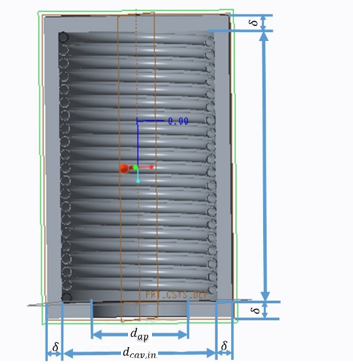
\includegraphics[width = 0.8\textwidth]{graphics/dishReceiver}
	\caption{Structure of the dish receiver}
	\label{fig:dishReceiver}
\end{center}
\end{figure}
Ma conducted tests to determine the free convection losses from the receiver for six alternative setups, and the data were consistent with Stine and McDonald's free convection correlation\cite{Ma1993}. It is assumed that forced convection is independent of free convection in the receiver, so the total convection losses can be represented as the sum of the free and forced convection losses as shown in Figure~\ref{fig:thermal-lose}.

\begin{equation}
	q_{con,tot} = q_{con,free} + q_{con,forced}
\end{equation}

\noindent \begin{figure}[htbp]
\begin{center}
	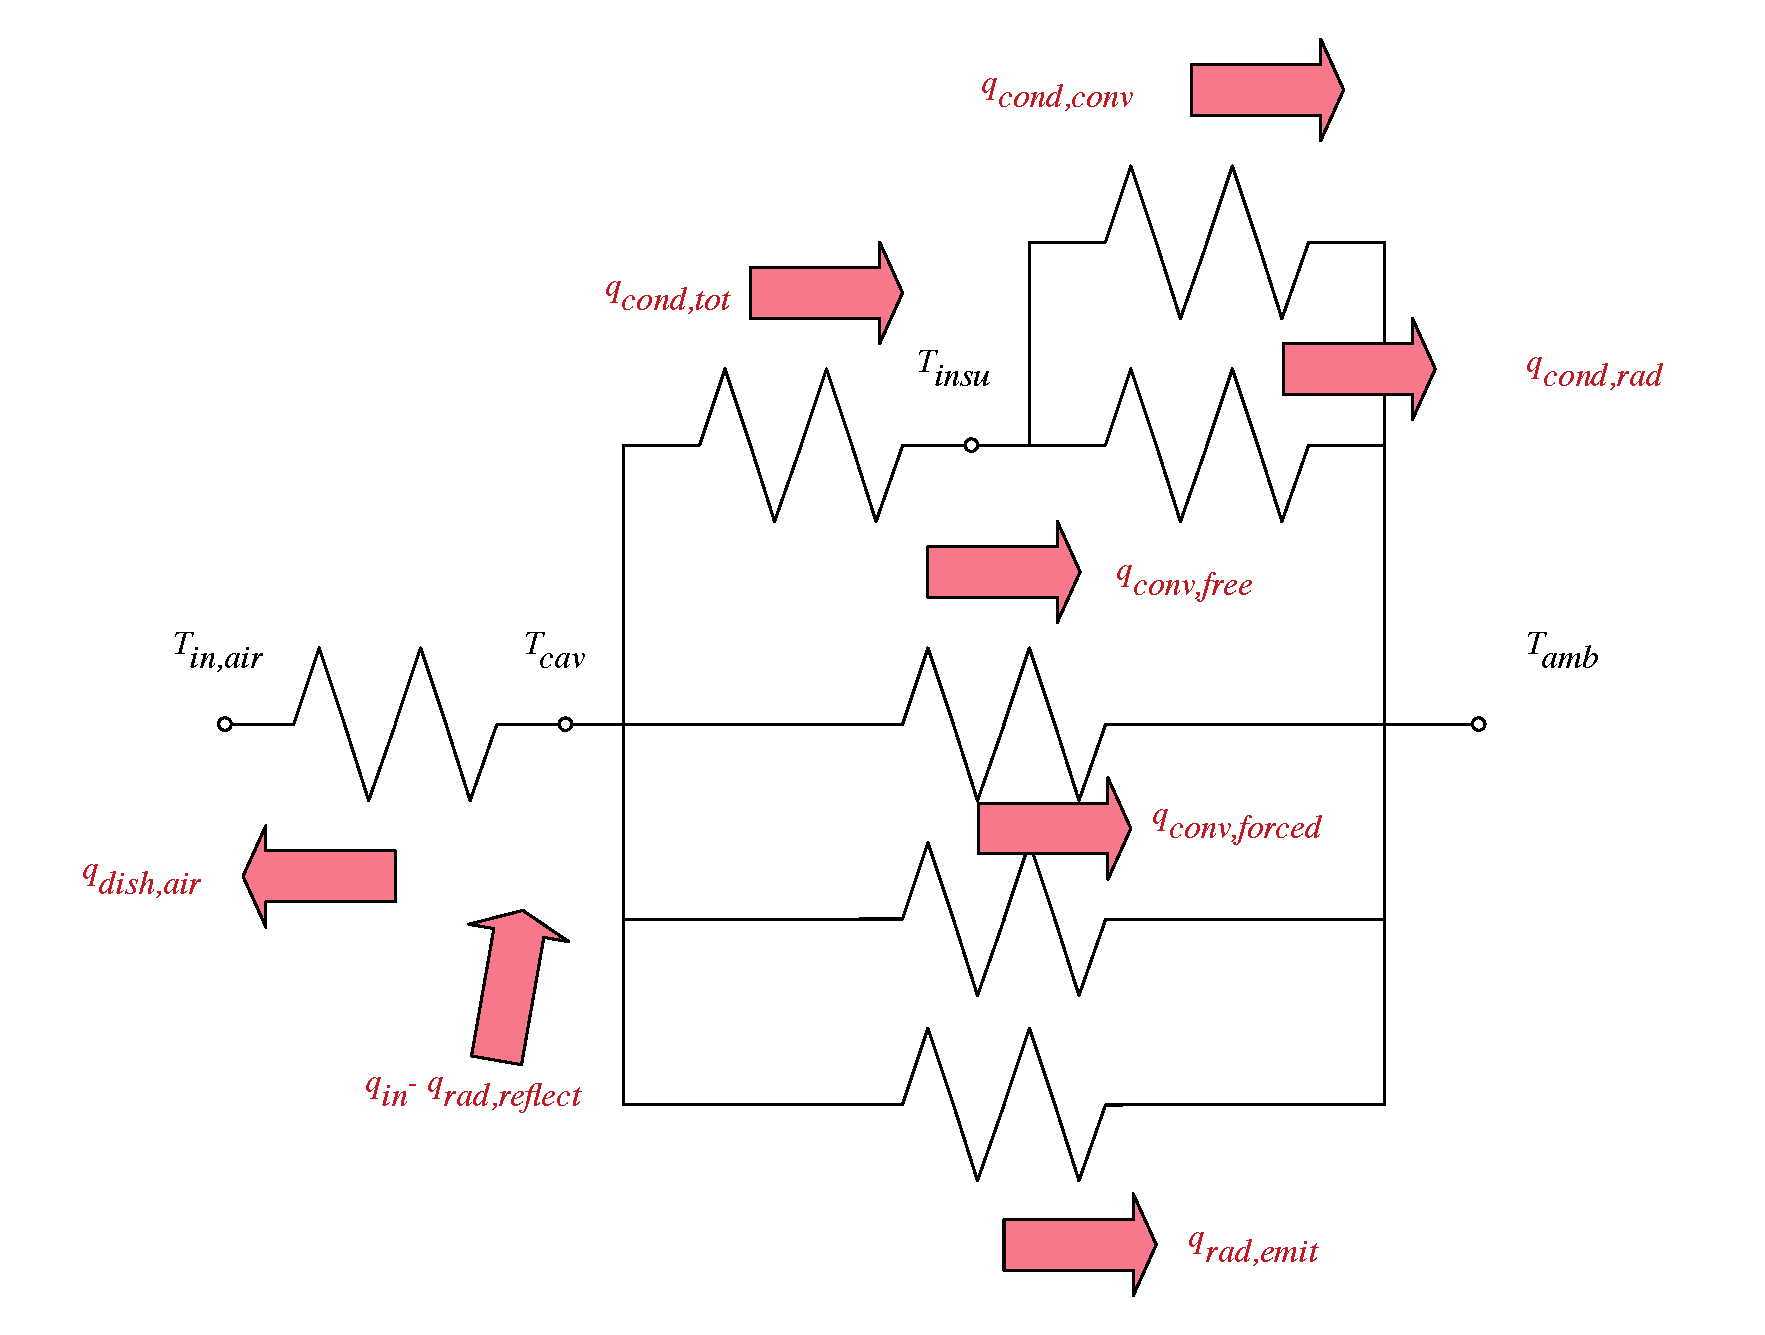
\includegraphics[width = 0.8\textwidth]{./graphics/thermalLosses}
	\caption{Heat network of dish receiver}
	\label{fig:thermal-lose}
\end{center}
\end{figure}
\begin{equation}
q_{in}\nomenclature{$q_{in}$}{Solar energy launched into dish receiver aperture, W} = q_{rad,reflect}\nomenclature{$q_{rad,reflect}$}{Reflected radiation}+q_{dish,air}\nomenclature{$q_{dish,air}$}{Energy absorbed by air in the dish collector}+(q_{cond,tot}\nomenclature{$q_{cond,tot}$}{Total conduction loss}+q_{conv,tot}\nomenclature{$q_{conv,tot}$}{Total convection loss}+q_{rad,emit}\nomenclature{$q_{rad,emit}$}{Radiation emitted by dish receiver})\label{eq:q_in sum}
\end{equation}

A dish collector product of SES\nomenclature[C]{SES}{Stirling Energy System} used in Fraser's paper, which is also used in this system, and its parameters are listed in Table~\ref{tab:dishReceiver}.\cite{Fraser2008} 

\begin{table}[htbp]
	\caption{Parameters of the dish receiver}
	\begin{center}
	\begin{tabular}{cc}
		\toprule
		Parameters	&	Value\\
		\midrule
		$d_{cav}$	&	0.46 m\\
		$\delta_{insu}$	&	0.075 m\\
		$l_{cav}$	&	0.23 m\\
		$d_{cav}$	&	0.184 m\\
		$\lambda_{insu}$	&	0.06 W/(m$\cdot$K)\\
		$\epsilon_{insu}$	&	0.6\\
		$\alpha_{cav}$	&	0.87\\
		$\delta_a$	&	0.005 m\\
		$d_{i,air}$	&	0.07 m\\
		$\theta_{dish}$	&	45$^\circ$\\
		$\gamma$	&	0.97\\
		$\eta_{shading}$	&	0.95\\
		$\rho$	&	0.91\\
		\bottomrule
	\end{tabular}
	\end{center}
	\label{tab:dishReceiver}
\end{table}
$q_{in}$ can be obtained by
\begin{equation}
q_{in}=DNI\cdot A_{dishCollector}\gamma\eta_{shading}\rho\label{eq:q_in}
\end{equation}



\clearpage
\bibliography{./bibliography/CascadeSystem}
\bibliographystyle{unsrt}

\end{document}